%%%%%%%%%%%%%%%%%%%%%%%%%%%%%%%%%%%%%%%%%%%%%%%%%%%%%%%%%%%%%%%%%%%%%%%%%%%%%%%%
%2345678901234567890123456789012345678901234567890123456789012345678901234567890
%        1         2         3         4         5         6         7         8
\documentclass[letterpaper, 10 pt, conference]{ieeeconf}  % Comment this line out
                                                          % if you need a4paper
%\documentclass[a4paper, 10pt, conference]{ieeeconf}      % Use this line for a4

\usepackage{float}
                                                          % paper
% uso paquete bookmark para tener bien los outlines.
\usepackage{bookmark}

% Configuro el idioma.
\usepackage[utf8]{inputenc} % Importante para mantener acentos.
\usepackage[spanish, activeacute]{babel} % Requiere: texlive-lang-spanish. Por primera vez hay que ejecutar: texconfig init> log

% Paquete para poder usar acentos en $$.
\usepackage{mathtools}
%\setmathfont{XITS math}

% Para los diagramas de flujo
\usepackage{tikz}
\usetikzlibrary{shapes.geometric, arrows}

% Elementos del diagrama
\tikzstyle{startstop} = [rectangle, rounded corners, 
minimum width=6em, 
minimum height=2em,
text centered, 
draw=black, 
fill=red!30]

\tikzstyle{io} = [trapezium, 
trapezium stretches=true, % A later addition
trapezium left angle=70, 
trapezium right angle=110, 
minimum width=6em, 
minimum height=2em, text centered, 
draw=black, fill=blue!30]

\tikzstyle{block} = [rectangle, 
minimum width=8em, 
minimum height=3em, 
text centered, 
text width=7.5em, 
draw=black, 
fill=white!30]

\tikzstyle{def} = [rectangle, 
minimum width=14em, 
minimum height=3em, 
text centered, 
text width=12em, 
draw=black, 
fill=purple!30]

\tikzstyle{swap_proccess} = [rectangle, 
minimum width=8em, 
minimum height=2em, 
text centered, 
text width=8em, 
draw=black, 
fill=orange!30]

\tikzstyle{process} = [rectangle, 
minimum width=6em, 
minimum height=2em, 
text centered, 
text width=6em, 
draw=black, 
fill=orange!30]

\tikzstyle{decision} = [diamond, 
minimum width=6em, 
minimum height=6em, 
text centered, 
draw=black, 
fill=green!30]
\tikzstyle{arrow} = [thick,->,>=stealth]

\usepackage{siunitx}

% package to get \url
\usepackage{hyperref}
\hypersetup{
  colorlinks=true,
  linkcolor=magenta,
  filecolor=magenta,
  citecolor=magenta,      
  urlcolor=magenta,
}

% Graficos electrónicos
\usepackage[RPvoltages]{circuitikz}

\IEEEoverridecommandlockouts                              % This command is only
                                                          % needed if you want to
                                                          % use the \thanks command
\overrideIEEEmargins
% See the \addtolength command later in the file to balance the column lengths
% on the last page of the document

\usepackage{graphicx}
\usepackage{graphics}

% styling for matlab/octave code.
\usepackage{matlab-prettifier}
% Configuracion, con esto puede agregar ñ.
\lstset{
  literate={ñ}{{\~n}}1
}

\usepackage{listings}

% The following packages can be found on http:\\www.ctan.org
%\usepackage{graphics} % for pdf, bitmapped graphics files
%\usepackage{epsfig} % for postscript graphics files
%\usepackage{mathptmx} % assumes new font selection scheme installed
%\usepackage{times} % assumes new font selection scheme installed
\usepackage{amsmath} % assumes amsmath package installed
%\usepackage{amssymb}  % assumes amsmath package installed

\title{\LARGE \bf Entregable Trabajo Práctico N° 4}

\author{
  Tom\'as Vidal\\
  {\it Sistemas Operativos y Redes}\\
  {\it Facultad de Ingenier\'ia, UNLP, La Plata, Argentina.}\\
  {\it 28 de Noviembre, 2024.}
}                                            % <-this % stops a space


% comienzo

% INTRO


% Figura
\newcommand{\image}[2] {
  \begin{figure}[H]
    \centering
    \includegraphics[width=0.43\textwidth]{./#1.png}
    \caption{#2}
    \label{fig:#1}
  \end{figure}
}

% Codigo
% \begin{lstlisting}[style=Matlab-editor]
% % el código va aca
% dispc("HELLO WORLD");
% \end{lstlisting}

\begin{document}
\maketitle
\thispagestyle{empty}
\pagestyle{empty}

\section{Redes presentadas}
En la figura \ref{fig:red_dada} se muestra la topología de las redes que fueron asignadas. Para hacer el análisis de la misma se empleó la dirección IP asignada \textit{181.29.152.0} con CIDR\footnote{El enrutamiento entre dominios sin clases (CIDR) es un método de asignación de direcciones IP que mejora la eficiencia del enrutamiento de datos en Internet} \textit{22}.

\begin{figure}[H]
	\centering
	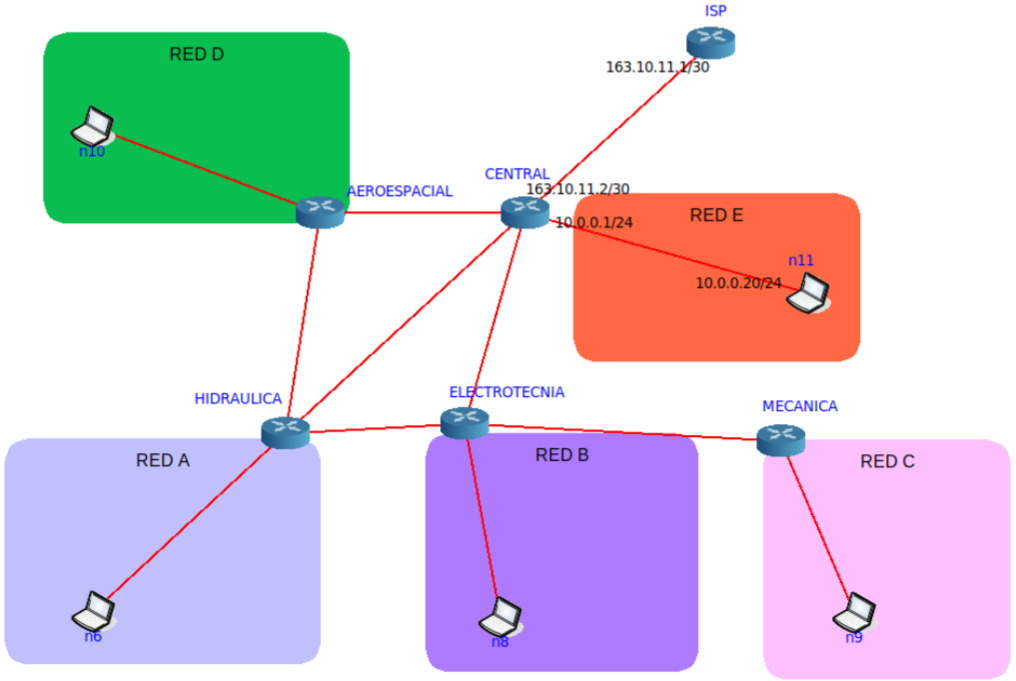
\includegraphics[width=0.43\textwidth]{./Imagenes/red_topologia.png}
	\caption{Topología de la red dada}
	\label{fig:red_dada}
\end{figure}

\subsection{Clase de la dirección IP}
La dirección IP \textit{163.10.11.2} pertenece a la \textbf{clase B}. Esto se debe a que el primer octeto (\textit{163}) se encuentra en el rango de direcciones de \textbf{clase B}, que va desde \textit{128} hasta \textit{191}.

En las direcciones de \textbf{clase B}, el prefijo por defecto es \textit{/16} (es decir, una máscara de red \textit{255.255.0.0}). Esto significa que los primeros 16 bits representan la parte de red, y los 16 bits restantes están destinados a los hosts. Sin embargo, en este caso, el prefijo asignado es \textit{/30}, lo cual indica que la red ha sido subneteada (\textit{subnetting}\footnote{El término \textit{subnetting} hace referencia a la subdivisión de una red en varias subredes}). Esto implica que se está utilizando un rango más pequeño de direcciones IP para optimizar el uso de la red (sólo se disponen de 2 hosts). Este \textit{subnetting} se da entre el ISP y el router que contiene a todas las redes, por eso no se necesitan más dispositivos.

\subsection{Cantidad de hosts de la red principal}
La red a la que se la denomina \textit{principal}, contiene a las redes \textbf{Hidráulica, Aeroespacial, Electrónica y la red E}, y tiene un CIDR de \textit{/24}, lo que deja disponibles 8 bits para los hosts. Los 8 bits se obtienen de saber que el total de bits para IPv4 es de 32, entonces:

\begin{equation*}
	32 - 24 = 8
\end{equation*}

El número de direcciones que se pueden asignar a hosts se calcula como:

\begin{equation*}
	2^{8} - 2 = 254
\end{equation*}

Se restan 2 direcciones porque:
\begin{itemize}
	\item Una se utiliza para la dirección de \textbf{red}.
	\item Otra se utiliza para la dirección de \textbf{broadcast}.
\end{itemize}

Por lo tanto la cantidad máxima de hosts que puede contener la red princiapl es de \textbf{254 hosts}. De los cuales

\subsection{Hosts en las subredes}

Como se reservan IPs para \textbf{Hidráulica, Aeroespacial, Electrónica, default y broadcast} quedan disponibles para la \textbf{red E} un total de 249 hosts:

\begin{equation*}
	254 - 5 = 249
\end{equation*}

\section{Asignación de las IPs}

Para hacer la asignación se tiene en cuenta que la red tiene una IP default \textit{10.0.0.1} con máscara \textit{255.255.255.0}:

% \begin{itemize}
%   \item \textbf{Hidráulica:} \textit{10.0.0.128/25}, 126 hosts. \textit{Desde 10.0.0.129 hasta 10.0.0.254}
%   \item \textbf{Aeroespacial:} \textit{10.0.2.0/23}, 510 hosts. \textit{Desde 10.0.1.0 hasta 10.0.3.0}
%   \item \textbf{Electrotecnia:} \textit{10.0.3.0/23}, 510 hosts. \textit{Desde 10.0.3.0 hasta 10.0.5.0}
%   {
%     \begin{itemize}
%       \item \textbf{Mecánica:} \textit{10.0.3.0/26}, 62 hosts.
%     \end{itemize}
%   }
% \end{itemize}

\begin{table}[H]
	\centering
	\begin{tabular}{|l|l|c|c|l|l|}
		\hline
		\textbf{Red}  & \textbf{IP} & \textbf{CIDR} & \textbf{Máscara} & \textbf{Rango}          \\ \hline
		Hidráulica    & 10.0.0.128  & /25           & 255.255.255.128  & 10.0.0.129 - 10.0.0.254 \\ \hline
		Aeroespacial  & 10.0.2.0    & /23           & 255.255.254.0    & 10.0.2.1 - 10.0.3.254   \\ \hline
		Electrotecnia & 10.0.4.0    & /23           & 255.255.254.0    & 10.0.4.1 - 10.0.5.254   \\ \hline
		Mecánica      & 10.0.5.192  & /26           & 255.255.255.192  & 10.0.5.193 - 10.0.5.254 \\ \hline
	\end{tabular}
	\caption{Alojamiento de direcciones}
	\label{tab:subnet_allocation}
\end{table}

\section{Configuración de las tablas de ruteo}

Se emplearon los siguientes comandos que permiten configurar las \textit{tablas de ruteo}\footnote{Routing tables. Son las tablas que permiten redirijir los paquetes en los routers para que tengan el comportamiento deseado.}:

\begin{itemize}
	\item ip addr add \textit{'dirección IP'} dev \textit{'interfaz'}
	\item ip route add \textit{'dirección IP'} via \textit{'dirección IP'}
	\item ping \textit{'dirección IP'}
\end{itemize}

Lo que se hizo fué abrir terminales en los diferentes \textit{routers}, y en ellos se configuraron las tablas como se muestra a continuación en las imágenes:

\begin{figure}[H]
	\centering
	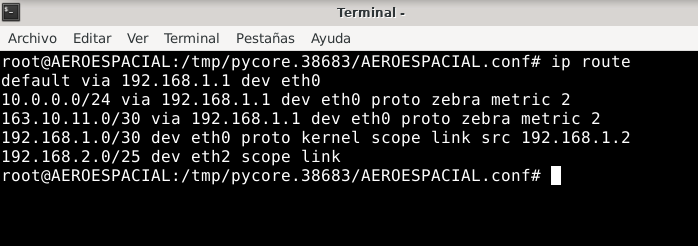
\includegraphics[width=0.43\textwidth]{./Imagenes/table1_AERO.png}
	\caption{Tablas de ruteo del router de aeroespacial}
	\label{fig:table_aero1}
\end{figure}

\section{Implementación del servidor TCP}

El protocolo TCP descompone los datos en paquetes y los reenvía a la capa del protocolo de Internet (IP) para garantizar que cada mensaje llegue a su ordenador de destino. El estado actual de desarrollo del protocolo TCP permite establecer una conexión entre dos puntos terminales en una red informática común que posibilite un intercambio mutuo de datos. En este proceso, cualquier pérdida de datos se detecta y resuelve, por lo que se considera un protocolo fiable. \\

La secuencia específica para establecer una conexión con el protocolo TCP es la siguiente:

\begin{enumerate}
	\item En el primer paso, el cliente que desea establecer la conexión envía al servidor un paquete SYN o segmento SYN (del inglés synchronize = “sincronizar”) con un número de secuencia individual y aleatorio. Este número garantiza la transmisión completa en el orden correcto (sin duplicados).
	\item Si el servidor ha recibido el segmento, confirma el establecimiento de la conexión mediante el envío de un paquete SYN-ACK (del inglés acknowledgement = “confirmación”) incluido el número de secuencia del cliente después de sumarle 1. De forma adicional, transmite un número de secuencia propio al cliente.
	\item Para finalizar, el cliente confirma la recepción del segmento SYN-ACK mediante el envío de un paquete ACK propio, que en este caso cuenta con el número de secuencia del servidor después de sumarle 1. En este punto también puede transmitir ya los primeros datos al servidor.
\end{enumerate}

\begin{figure}[H]
	\centering
	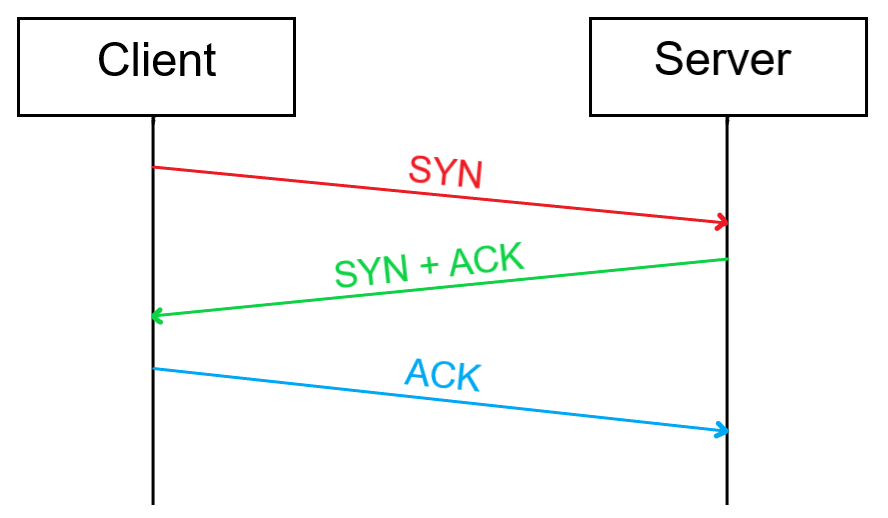
\includegraphics[width=0.43\textwidth]{./Imagenes/tcp_ack.png}
	\caption{Diagrama de la sincronización del TCP}
	\label{fig:tcp_ack}
\end{figure}

\subsection{Cabecera TCP}

\begin{figure}[H]
	\centering
	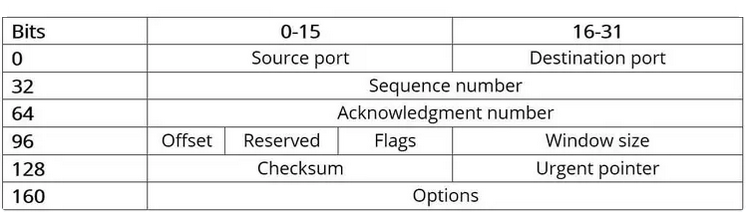
\includegraphics[width=0.43\textwidth]{./Imagenes/TPC_header.png}
	\caption{Estructura de la cabecera TCP}
	\label{fig:tcp_header}
\end{figure}



\end{document}